%
% Documento: Fundamentação Teórica
%

\chapter{Fundamentação Teórica}
\label{chap:fundamentacaoTeorica}

A seguir ilustra-se a forma de incluir figuras, tabelas, equações, siglas e símbolos no documento, obtendo indexação automática em suas respectivas listas. A numeração sequencial de figuras, tabelas e equações ocorre de modo automático. Referências cruzadas são obtidas através dos comandos \verb#\label{}# e \verb#\ref{}#. Por exemplo, não é necessário saber que o número deste capítulo é \ref{chap:fundamentacaoTeorica} para colocar o seu número no texto. Isto facilita muito a inserção, remoção ou relocação de elementos numerados no texto (fato corriqueiro na escrita e correção de um documento acadêmico) sem a necessidade de renumerá-los todos.

Este modelo prove um arquivo \textit{makefile}, portanto, para gerar este documento no formato PDF, basta apenas executar o comando {\ttfamily make all} no linux. Para limpar os arquivos temporários, basta digitar o comando {\ttfamily make clean}.

\section{Figuras e gráficos}
\label{sec:figuras}

Abaixo é apresentado um exemplo de figura e de gráfico. A figura \ref{fig:kdtree} aparece automaticamente na lista de figuras e o gráfico \ref{chr:buscaimg} aparece automaticamente na lista de gráficos. Para uso avançado de imagens no LATEX, recomenda-se a consulta de literatura especializada \cite{Goossens2007}.

\begin{figure}[!htb]
	\centering
	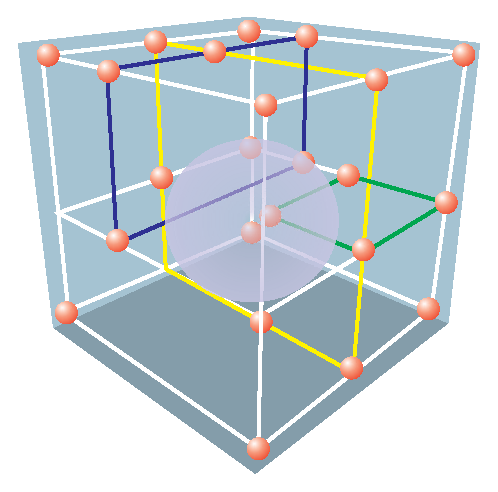
\includegraphics[width=0.3\textwidth]{./figuras/figkdtree.eps}
	\caption{Exemplo da estrutura de uma árvore KD}
	\fonte{\cite{CELSO2012}}
	\label{fig:kdtree}
\end{figure}

\begin{grafico}[!htb]
	\centering
	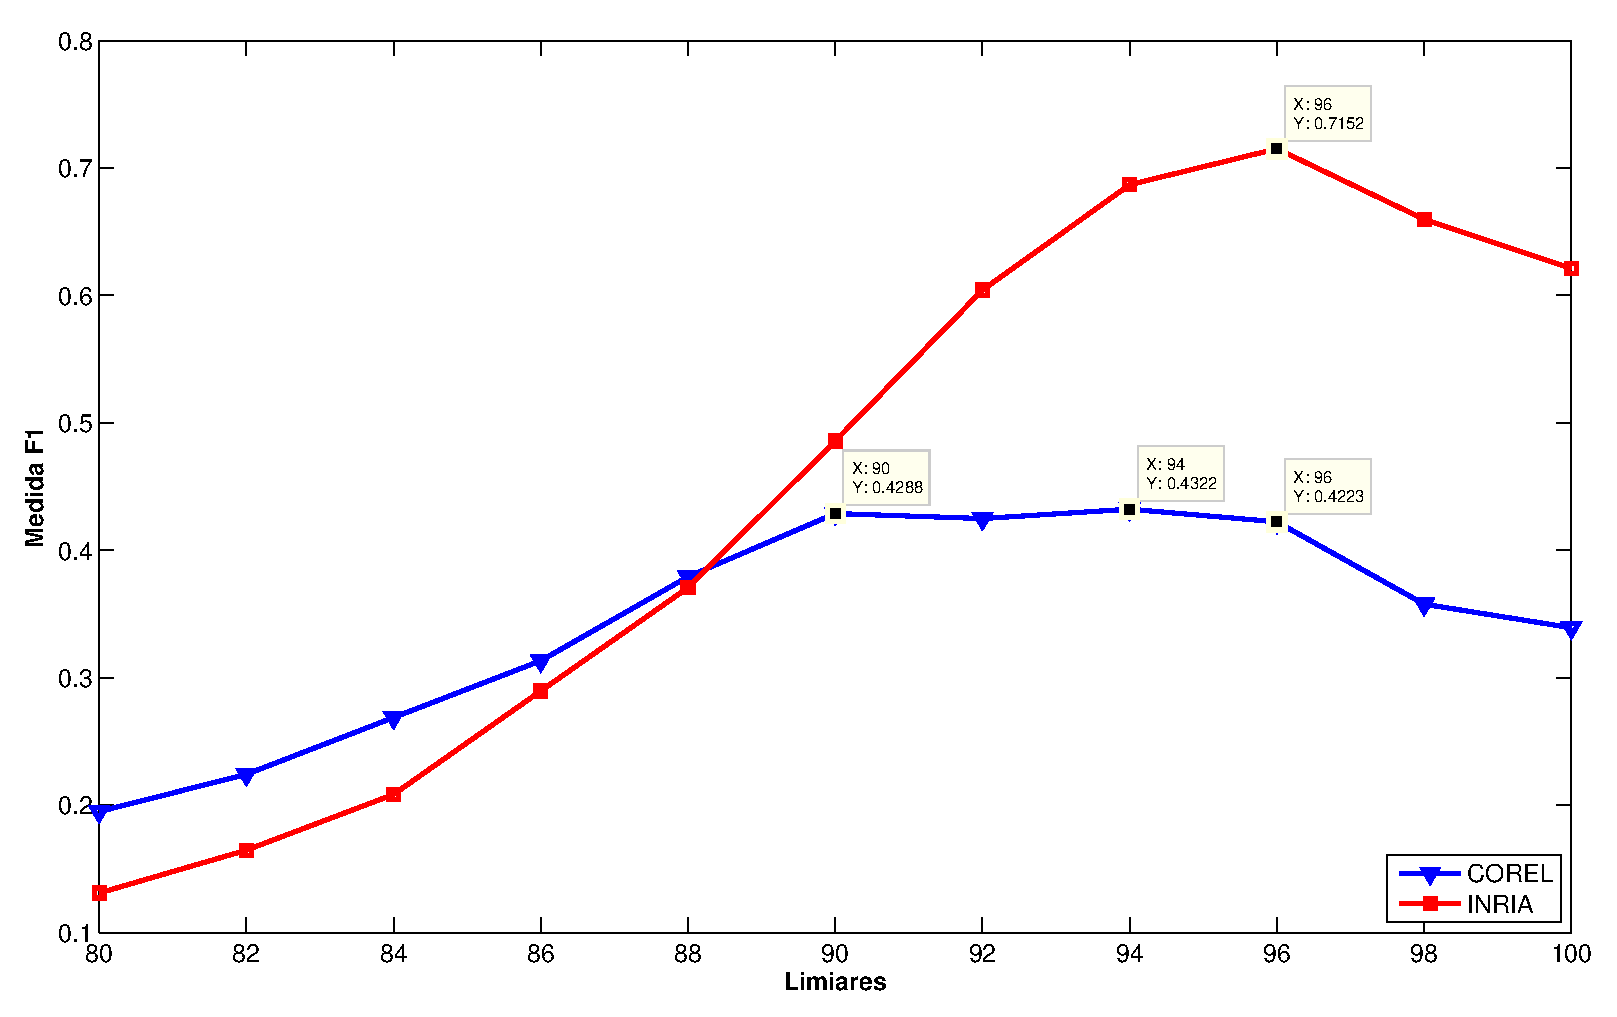
\includegraphics[width=0.7\textwidth]{./graficos/buscaimg.eps}
	\caption[Resultado da busca por imagem]{Resultado da busca por imagem.}
	\label{chr:buscaimg}
\end{grafico}

\section{Quadros e Tabelas}
\label{sec:tabelas}

Também é apresentado o exemplo do quadro \ref{qua:vertices} e da tabela \ref{tab:correlacao}, que aparece automaticamente na lista de tabelas. Informações sobre a construção de tabelas no LATEX podem ser encontradas na literatura especializada \cite{Lamport1986,Buerger1989,Kopka2003,Mittelbach2004}.

\begin{quadro}[!htb]
	\centering
	\begin{tabular}{|c|c|c|} \hline
		\multirow{2}{32mm}{Vértices Retirados} &\multicolumn{2}{|c|}{Componentes Excluídos} \\ \cline{2-3}
		&Quantidade &Vértices do maior componente\\ \hline\hline
		Original &0        &- \\ \hline
		1\%      &4        &3 \\ \hline
		5\%      &14       &3 \\ \hline
		10\%     &31       &5 \\ \hline
		20\%     &66       &5 \\ \hline
		30\%     &94       &5 \\ \hline
		40\%     &110      &5 \\ \hline
		50\%     &166      &5 \\ \hline
		75\%     &352      &6 \\ \hline
		90\%     &688      &19 \\ \hline
	\end{tabular}
	\caption[Componentes desconectados na remoção híbrida]{Componentes desconectados na remoção híbrida\label{qua:vertices}}
\end{quadro}


Muitos confundem, mas existe diferença entre tabelas e quadros.
Um quadro é formado por linhas horizontais e verticais,
sendo, portanto ``fechado''. Normalmente é usado
para apresentar dados secundários. Nada impede, porém,
que um quadro apresente resultados da pesquisa.
Um quadro normalmente apresenta resultados
qualitativos (textos). O número do quadro e o título
vêm acima do quadro, e a fonte, deve vir abaixo.
Uma tabela é formada apenas por linhas verticais, sendo,
portanto ``aberta''. Normalmente é usada para
apresentar dados primários, e geralmente vem nos
“resultados” e na discussão do trabalho. Nada
impede, porém, que uma tabela seja usada no
referencial teórico de um trabalho. Uma tabela
normalmente apresenta resultados quantitativos
(números). O número da tabela e o título vêm
acima da tabela, e a fonte, deve vir abaixo, como
no quadro.

Exemplos de tabelas:

\begin{table}[!htb]
	\centering
	\caption[Correlação de valores x e y]{Exemplo de uma tabela mostrando a correlação entre x e y.\label{tab:correlacao}}
	\begin{tabular}{cc}
		\hline 
		x & y \\
		\hline
		1 & 2 \\
		3 & 4 \\
		5 & 6 \\
		7 & 8 \\
		\hline 
	\end{tabular}
	\fonte{Autoria própria.}
\end{table}


\begin{table}[!htb]
	\centering
	\begin{tabular}{rrrrr}
		\toprule
			& Valores 1 & Valores 2 & Valores 3 & Valores 4 \\
		\midrule
			Caso 1 & 0,86 & 0,77 & 0,81 & 163 \\
			Caso 2 & 0,19 & 0,74 & 0,25 & 180 \\
			Caso 3 & 1,00 & 1,00 & 1,00 & 170 \\
		\bottomrule
	\end{tabular}
	\caption[Resultado dos testes]{Resultado dos testes.\label{tab:testes}}
\end{table}


\section{Equações}
\label{sec:equacoes}

A transformada de Laplace é dada na equação (\ref{eq:laplace}), enquanto a equação (\ref{eq:dft}) apresenta a formulação da transformada discreta de Fourier bidimensional\footnote{Deve-se reparar na formatação esteticamente perfeita destas equações.}.

\begin{equation}
	X(s) = \int\limits_{t = -\infty}^{\infty} x(t) \, \text{e}^{-st} \, dt
	\label{eq:laplace}
\end{equation}

\begin{equation}
	F(u, v) = \sum_{m = 0}^{M - 1} \sum_{n = 0}^{N - 1} f(m, n) \exp \left[ -j 2 \pi \left( \frac{u m}{M} + \frac{v n}{N} \right) \right]
	\label{eq:dft}
\end{equation}

\section{Siglas e símbolos}
\label{sec:siglas}

O pacote ABNTEX permite ainda a definição de siglas e símbolos com indexação automática através dos comandos \verb#\sigla{}{}# e \verb#\simbolo{}{}#. Por exemplo, o significado das siglas \sigla{ABNT}{Associação Brasileira de Normas Técnicas} e \sigla{DECOM}{Departamento de Computação} aparecem automaticamente na lista de siglas, bem como o significado dos símbolos\simbolo{$\lambda$}{comprimento de onda},\simbolo{$v$}{velocidade} e\simbolo{$f$}{frequência}aparecem automaticamente na lista de símbolos. Mais detalhes sobre o uso destes e outros comandos do ABNTEX são encontrados em sua documentação específica\cite{abnTeX2009}.

%\section{Algoritmos}
%\label{sec:algoritmos}
%
%Os algoritmos devem ser feitos segundo o modelo abaixo. 
%Para isso, utilizar o pacote  {\ttfamily algorithm2e} no início do arquivo principal como neste exemplo.
%
%\begin{algorithm}
%\KwIn{o número $n$ de vértices a remover, grafo original $G(V, E)$}
%\KwOut{grafo reduzido $G'(V,E)$}
% $removidos \leftarrow 0$ \\
% \While {removidos $<$ n } {
%   $v \leftarrow$ Random$(1, ..., k) \in V$ \\
%     \For {$u \in adjacentes(v)$} {
%	remove aresta (u, v)\\
%	$removidos \leftarrow removidos + 1$\\
%     }
%     \If {há  componentes desconectados} {
%	remove os componentes desconectados\\
%     }
%   }
%\caption{Algoritmo para remoção aleatória de vértices}
%\end{algorithm}
